\section{Experimental Results}
\label{sec:exp}

We train on the English-French parallel corpora from ACL WMT '14, which contains
348M words. To evaluate performance, we use the test set news-test-2014, also from
WMT '14, which contains 3003 new sentences. As a comparison metric, we additionally run the system presented by
\newcite{journals/corr/BahdanauCB14} using the same parameters and data. We ensure
that after our data transformation is applied, the resulting vocabulary also has size
30,000, matching the number used in their experiments. Taking inspiration from the standard Huffman encoding
priority queue algorithm, we construct the trees by the following method. First, we use
the formulas derived in the previous section to calculate the optimal number of
common words $W$ for each encoding scheme, using $V$ to be the vocabulary size of the original text and $K = 30000$.
We then find the $W$ words in the text with highest frequency and
apply the identity transformation to them. For the remaining words, we encode them
using a distinct symbol whose form matches the one prescribed for each
encoding scheme.\\

We use the RNNsearch-50 architecture from \newcite{journals/corr/BahdanauCB14} as
our black box machine translation system. We report results for this system alone,
as well as for each of our three encoding schemes, using the BLEU score metric for
ease of comparison with previously reported scores. Our results after training
for approximately 5 days are compiled in Table \ref{table:results} and Figure \ref{fig:graph}.\\

TODO: analyze results\\

\begin{table}
  \centering
  \vspace{8pt}
  \tabcolsep=0.11cm{
  \begin{tabular}{cccc}
    \toprule
      \textbf{Encoding} & \textbf{BLEU Score (5 days)}\\
    \midrule
      None & 0.2577\\
    \midrule
      Repeat-All & 0.2704\\
    \midrule
      Repeat-Symbol & TODO\\
    \midrule
      No-Repeats & TODO\\
    \bottomrule
  \end{tabular}}
  \caption{BLEU scores on detokenized test set for various encoding
    schemes after training for 5 days.}
  \label{table:results}
\end{table}

\begin{figure}
  \centering
  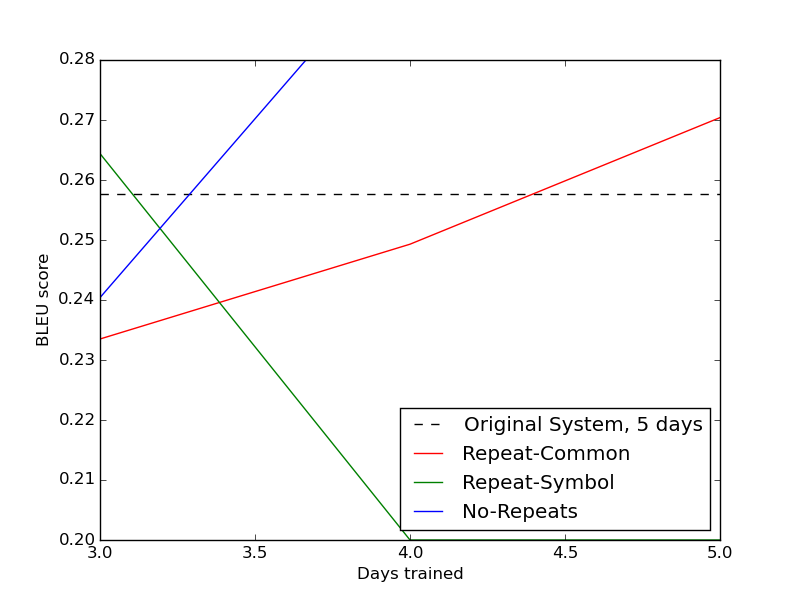
\includegraphics[scale=0.6]{images/graph.png}
  \caption{BLEU score after each day of training for each encoding scheme.}
  \label{fig:graph}
\end{figure}